% !TeX spellcheck = cs_CZ
{\tikzset{external/prefix={tikz/FYZII/}}
 \tikzset{external/figure name/.add={ch25_}{}}
%---------------------------------------------------------------------------------------------------
% file fey2ch25.tex
%---------------------------------------------------------------------------------------------------
%=========================== Kapitola Elektrodynamika v relativistickém zápisu =====================
\chapter{Elektrodynamika v relativistickém zápisu}\label{fyz:IIchaXXV}
\minitoc
  \section{Čtyřvektory}\label{fyz:IIchaXXVsecI}
  \section{Skalární součin}\label{fyz:IIchaXXVsecII}
  \section{Čtyřrozměrný gradient}\label{fyz:IIchaXXVsecIII}
  \section{Elektrodynamika v čtyřrozměrném zápisu}\label{fyz:IIchaXXVsecIV}
  \section{Čtyřpotenciál pohybujícího se náboje}\label{fyz:IIchaXXVsecV}
  \section{Invariance rovnic elektrodynamiky}\label{fyz:IIchaXXVsecVI}
  \section{Příklady a cvičení}\label{fyz:IIchaXXVsecVII}

    \begin{figure}[ht!] %\ref{fyz_fig600}
      \centering
      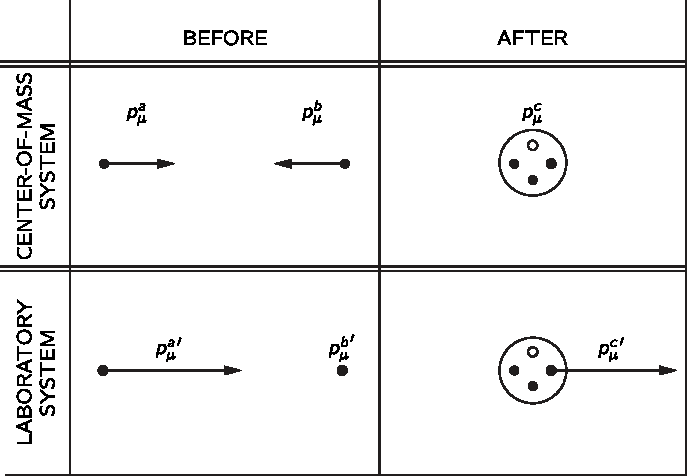
\includegraphics[width=0.7\linewidth]{fyz_fig600.pdf}
      \caption{
               (\cite[s.~707]{Feynman02})}
      \label{fyz_fig600}
    \end{figure}


    \begin{figure}[ht!] %\ref{fyz_fig601}
      \centering
      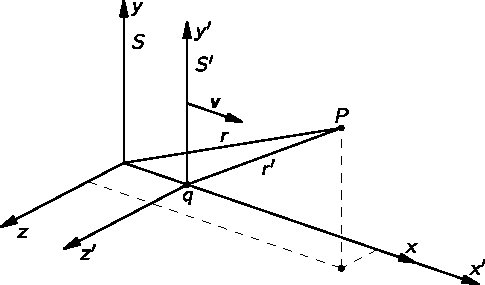
\includegraphics[width=0.7\linewidth]{fyz_fig601.pdf}
      \caption{
               (\cite[s.~707]{Feynman02})}
      \label{fyz_fig601}
    \end{figure}
    
} %tikzset
%---------------------------------------------------------------------------------------------------
\printbibliography[title={Seznam literatury},heading=subbibliography]
\addcontentsline{toc}{section}{Seznam literatury}